\فصل{روش آلیاس}
\lr{آلیاس}\footnote{\lr{alias}
این روش ، یک روش برای تولید کردن یک عدد تصادفی$x$ با داشتن یک بردار احتمال$ p_{0}, p_{1}, ..., p_{k}$  می‌باشد   . در این روش به یک جدول با اندازه$ O(K)$  نیاز داریم.  زمان مورد نیاز این روش  بعد از  انجام پیش محاسبات $ O(1)$ می باشد.
 این روش بر تئوری زیر استوار است :
هر بردار احتمال p_{0}, p_{1} , ..., p_{k -1}  را می توان به صورت مجموعه ای از زوج مرتب ها نمایش داد . 


در زیر چند تصویر که با استفاده از روش‌های مختلف بحث شده در این پروژه ساخته شده اند را مشاهد می‌کنید.

  
  \begin{figure}[!htb]
  	\minipage{0.48\textwidth}
  	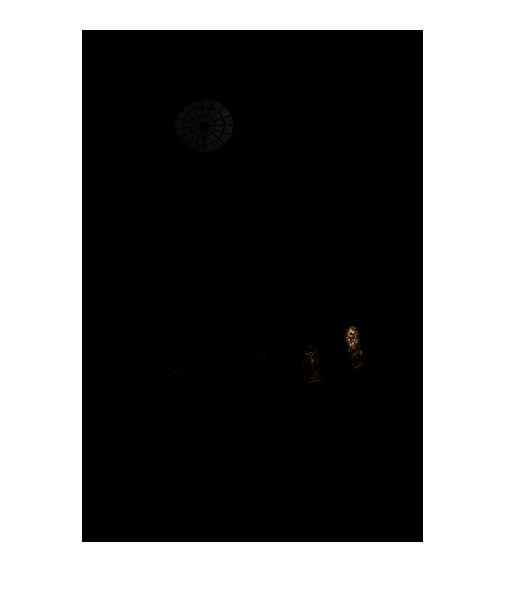
\includegraphics[width=\linewidth]{images/linearhdr1}
  	\caption{linear}\label{fig:logtonemap}
  	\endminipage\hfill
  	\minipage{0.48\textwidth}
  	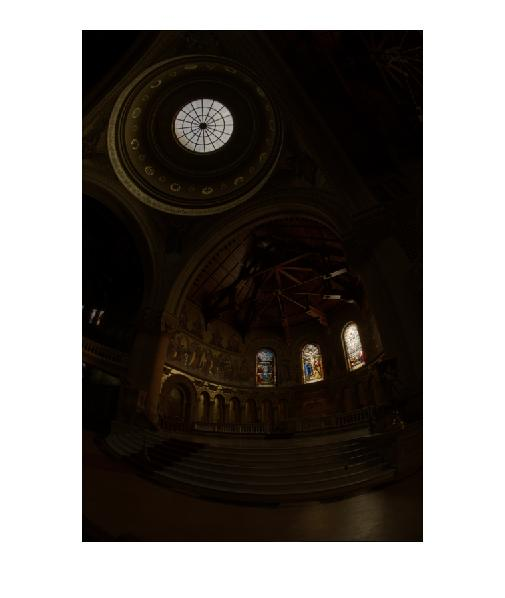
\includegraphics[width=\linewidth]{images/loghdr1}
  	\caption{logarithmic}\label{fig:lineartonemap}
  	\endminipage\hfill
  	% 	\centerline{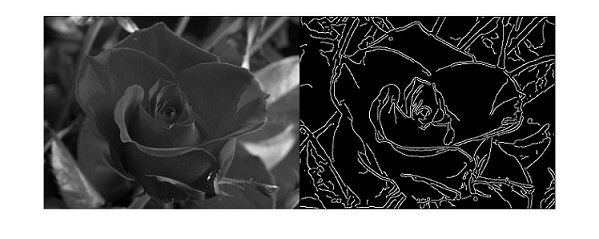
\includegraphics{images/cannyexample2}}
   \end{figure}
      
  \begin{figure}[!htb]
    \minipage{1\textwidth}
      	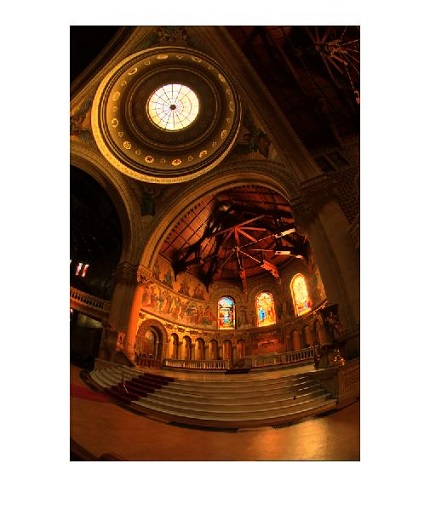
\includegraphics[width=\linewidth]{images/reinhardhdr1}
      	\caption{rainhard}\label{fig:logtonemap}
    \endminipage\hfill
      	% 	\centerline{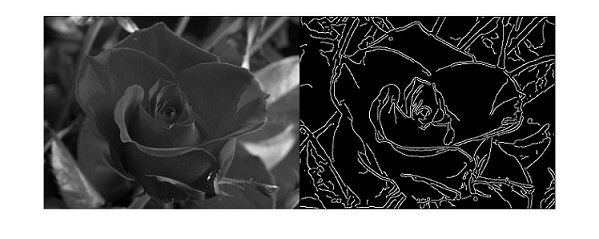
\includegraphics{images/cannyexample2}}
   \end{figure}
      
        
    \begin{figure}[!htb]
     \minipage{1\textwidth}
        	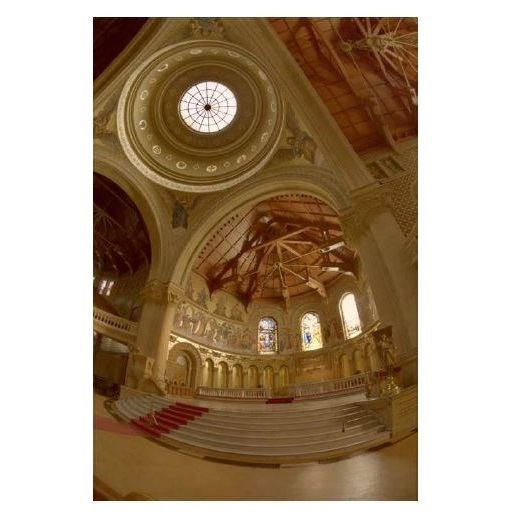
\includegraphics[width=\linewidth]{images/retinex3}
        	\caption{retinex}\label{fig:logtonemap}
      \endminipage\hfill
        	% 	\centerline{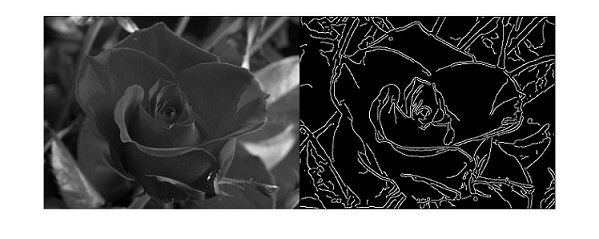
\includegraphics{images/cannyexample2}}
    \end{figure}
        
        
      \begin{figure}[!htb]
      	\minipage{0.48\textwidth}
      	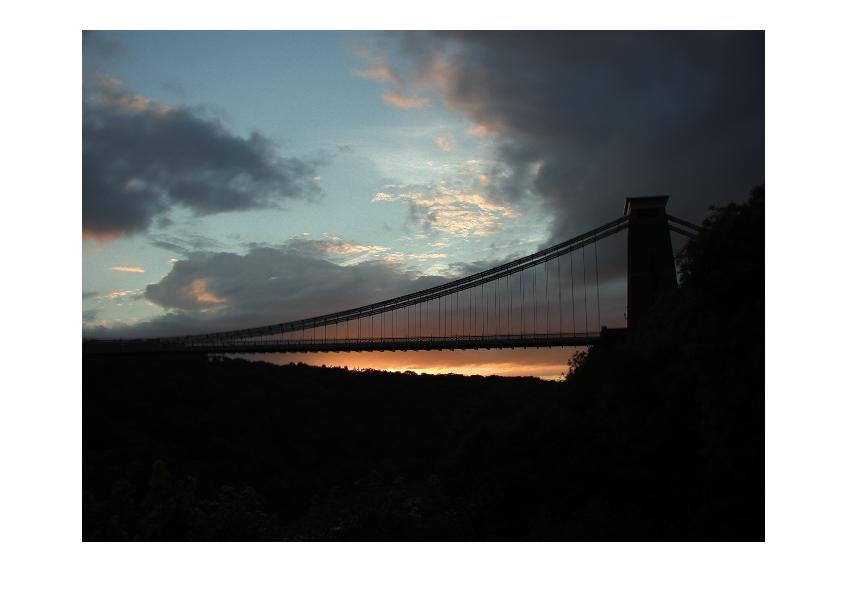
\includegraphics[width=\linewidth]{images/linearhdr3}
      	\caption{linear}\label{fig:logtonemap}
      	\endminipage\hfill
      	\minipage{0.48\textwidth}
      	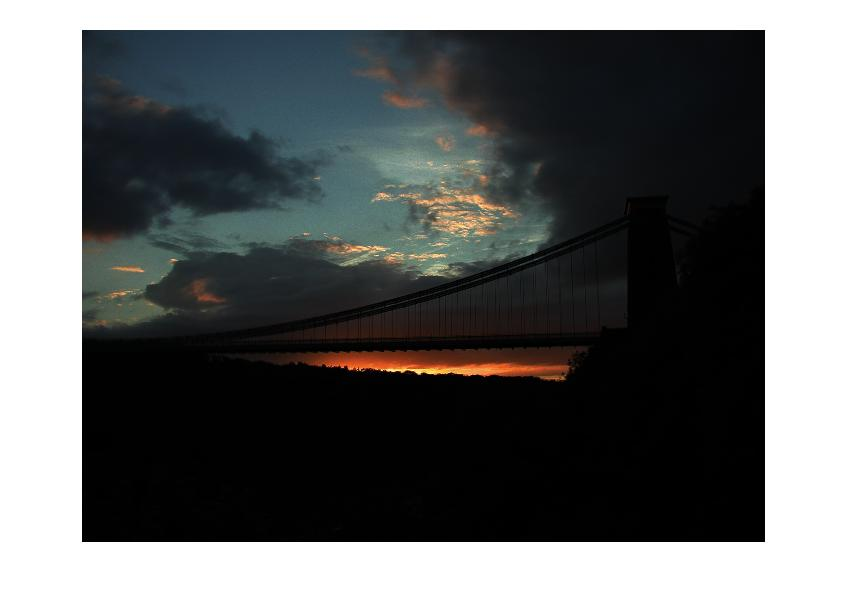
\includegraphics[width=\linewidth]{images/loghdr3}
      	\caption{logarithmic}\label{fig:lineartonemap}
      	\endminipage\hfill
      	% 	\centerline{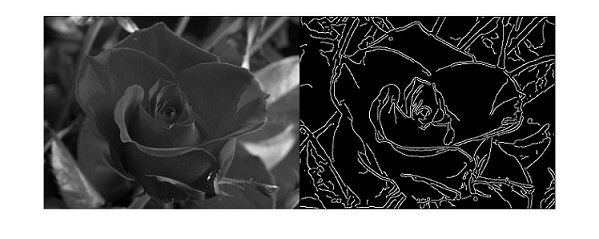
\includegraphics{images/cannyexample2}}
      \end{figure}
      
      \begin{figure}[!htb]
      	\minipage{1\textwidth}
      	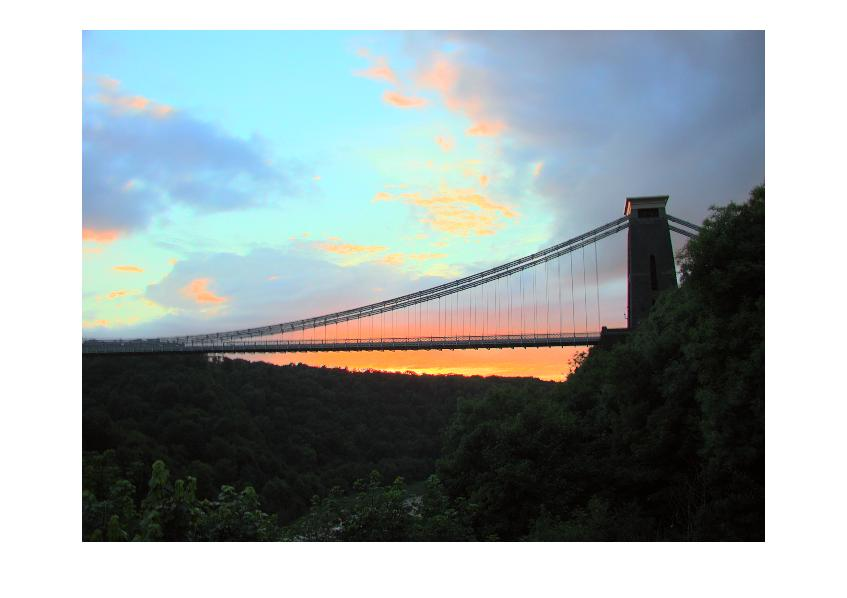
\includegraphics[width=\linewidth]{images/rainhardhdr3}
      	\caption{rainhard }\label{fig:logtonemap}
      	\endminipage\hfill
      	% 	\centerline{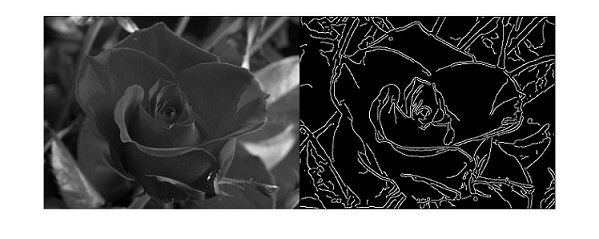
\includegraphics{images/cannyexample2}}
      \end{figure}
      
      
      \begin{figure}[!htb]
      	\minipage{1\textwidth}
      	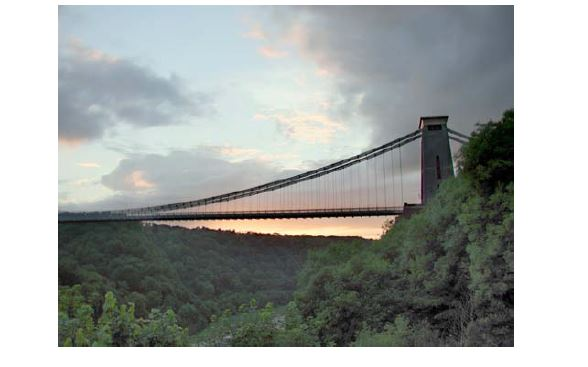
\includegraphics[width=\linewidth]{images/retinex1}
      	\caption{retinex}\label{fig:logtonemap}
      	\endminipage\hfill
      	% 	\centerline{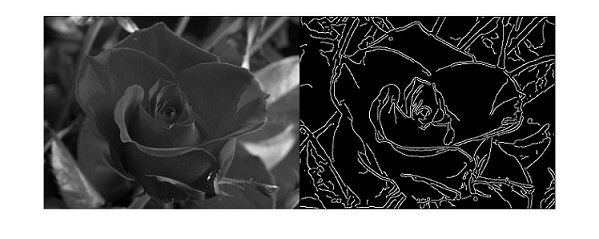
\includegraphics{images/cannyexample2}}
      \end{figure}
         